\documentclass[11pt,fleqn]{article}

\setlength {\topmargin} {-.15in}
\setlength {\textheight} {8.6in}

\usepackage{amsmath}
\usepackage{amssymb}
\usepackage{color}
\usepackage{tikz}
\usetikzlibrary{automata,positioning,arrows}
\usepackage{diagbox}
\usepackage{stackrel}

\newcommand{\be}{\begin{enumerate}}
\newcommand{\ee}{\end{enumerate}}

\begin{document}


\textbf{Exercise 3.3.38:} Fundamental theorem of rotations. Show that any BST can be transformed into
any other BST on the same set of keys by a sequence of left and right rotations.\\

\textbf{Solution}:

\begin{itemize}
	\item Recall that BSTs with rotation allow for the shifting of nodes.
	
	\item By doing these rotations a certain number of times, we can effectively change the shape of BSTs to the one of our own choice.
	
	\item For example, if repeated rotations occur, eventually certain sides of the tree and subtrees become null and we end up getting a LinkedList shown below.
\end{itemize}

\begin{center}
	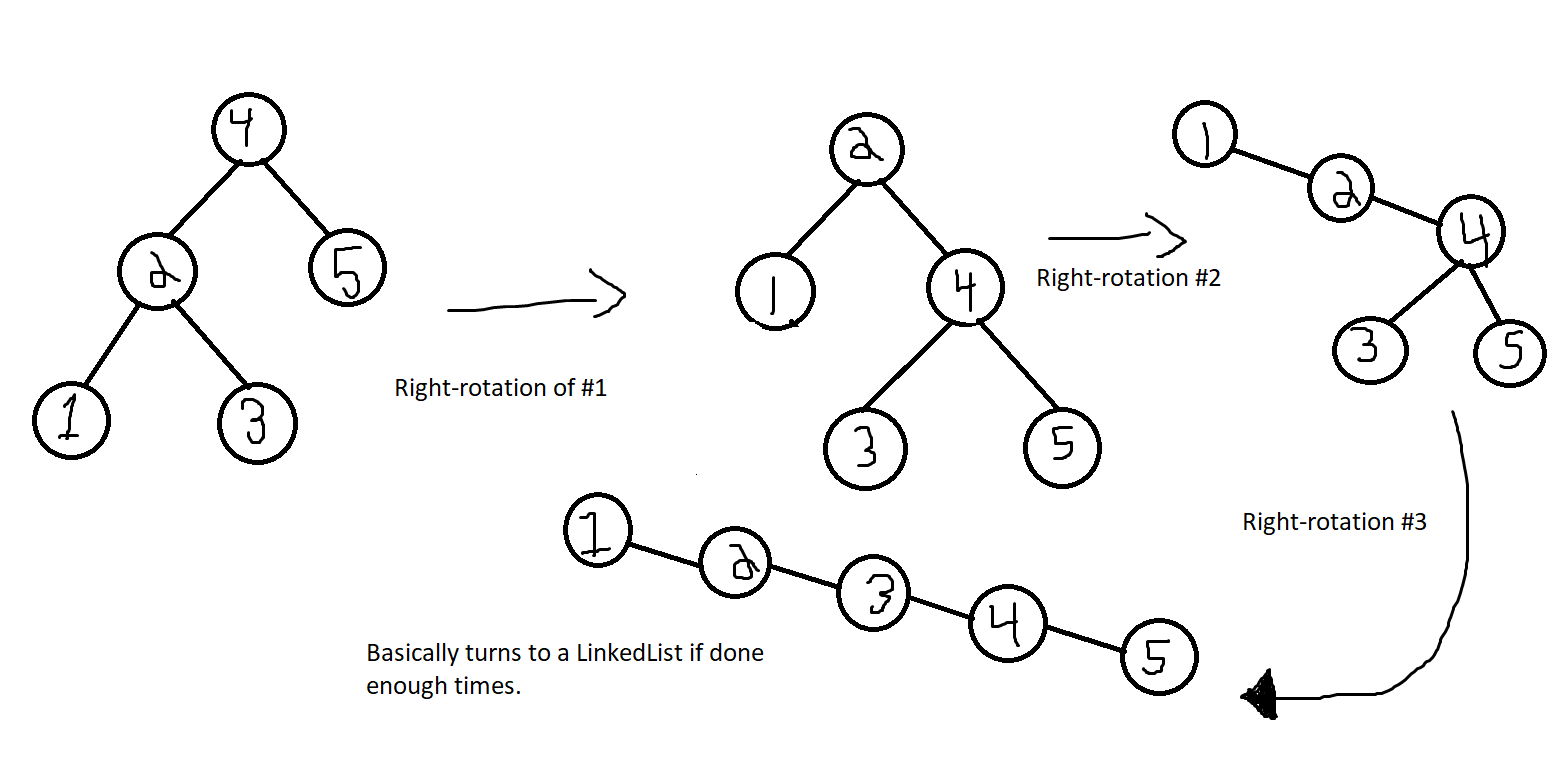
\includegraphics[scale=.45]{3.3.38.png}
\end{center}

\newpage
\textbf{Same idea for left-rotations:}
\begin{center}
	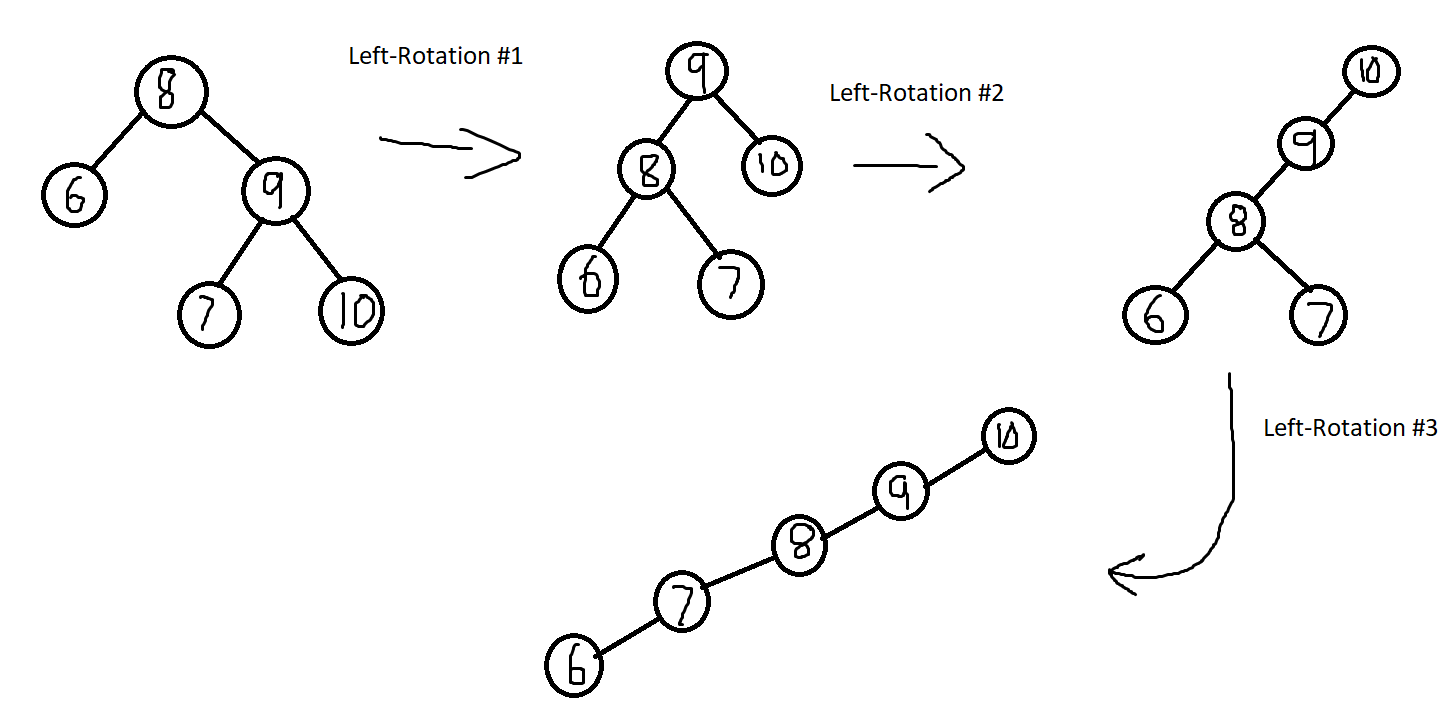
\includegraphics[scale=.5]{3.3.38-1.png}
\end{center}

So by showcasing how a BST can be converted to a single LinkedList, this clearly proves that we can create any BST with same set of keys by the sequence.


\end{document}
